\chapter{State of the Art Description}
\section{What are the main problems when creating exploded views?}

To create an exploded view,  a few considerations have to be made Li et al. provide a comprehensive list of these challenges in their 2008 paper\cite{proc:Li:2008:AGI}.\\
Most important of all is the question what Information should be transported with the image, what  the purpose of the illustration is. In essence what are the objects of interest that should attract the viewers attention? This usually is determined by preliminary definition of interesting features, definitions of parts, subsets of parts of the data or user interaction while viewing the graphic.
\subsection{Explosion direction}
Also one has to consider in which direction the parts should be displaced. 
\begin{quote}
Many objects have a canonical coordinate frame that may be defined by a number of factors, including symmetry , real-world orientation, and domain-specific conventions. In most exploded views, parts are exploded only along these canonical axes.\cite{proc:Li:2008:AGI}
\end{quote}
Especially if the graphic conveys technical instructions or how-things-work-descriptions descriptions these axes are usually the directions in which they are assembled \cite{Agra03} or - if applicable- the axis around which they rotate\cite{MitraYYLA13}.
If the interesting parts are inside a container that is also part of the object, this container is split and its segments are also exploded. In the most simple approach, which is what I implemented, the cutting plane is the normal plane of the explosion direction, with the center of the object's bounding box.
\begin{figure}[tb]
	\centering
	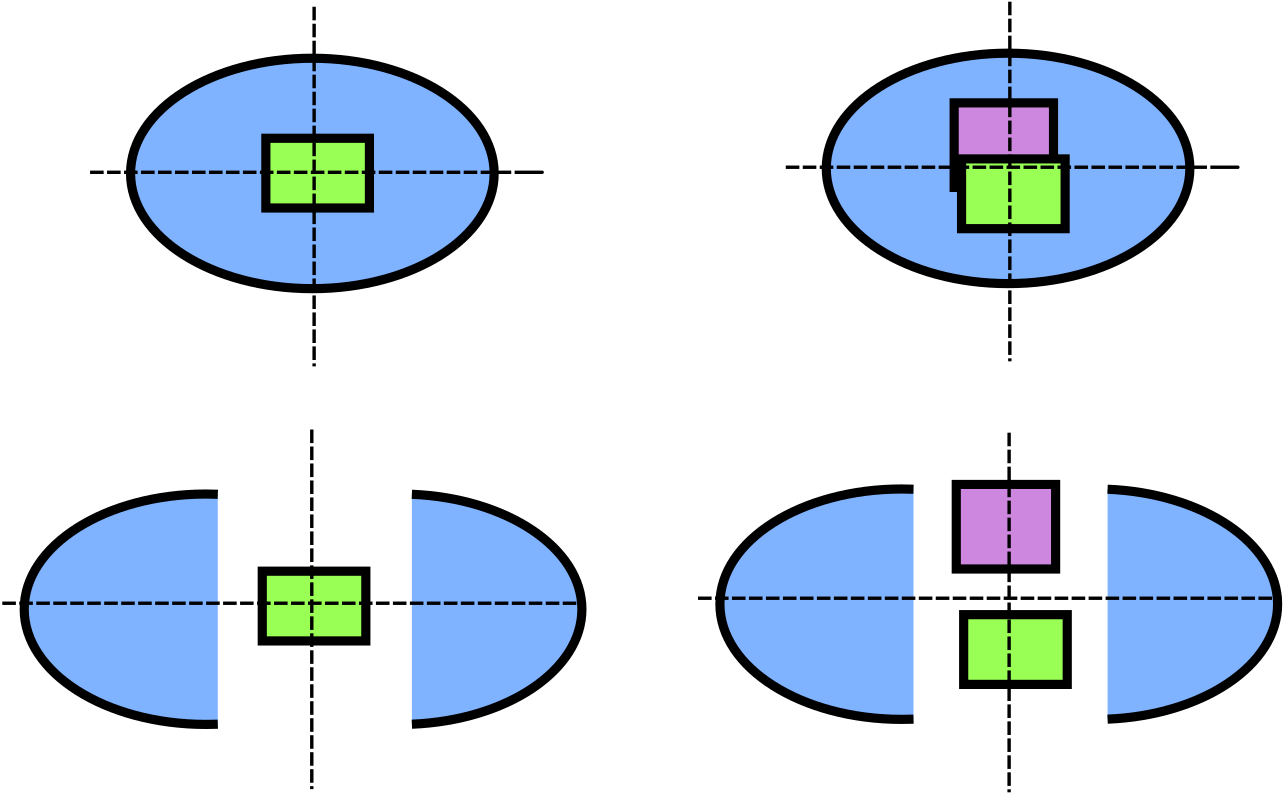
\includegraphics[width=0.9\textwidth]{chapters/figures/splitting}
	\caption{The object of interest is revealed by splitting its container and moving the two segments away from the object in the center.}
	\label{fig:splitting}
\end{figure}
\subsection{Part hierarchy}
Take for example an object that has a container and a lot of small parts that inside whose function should be clarified by exploding them in their canonical direction.  In this case it might be convenient to split and explode the container along a different axis than the internal parts to get a more compact visualization(see \ref{fig:axes}).\\
\begin{figure}[tb]
	\centering
	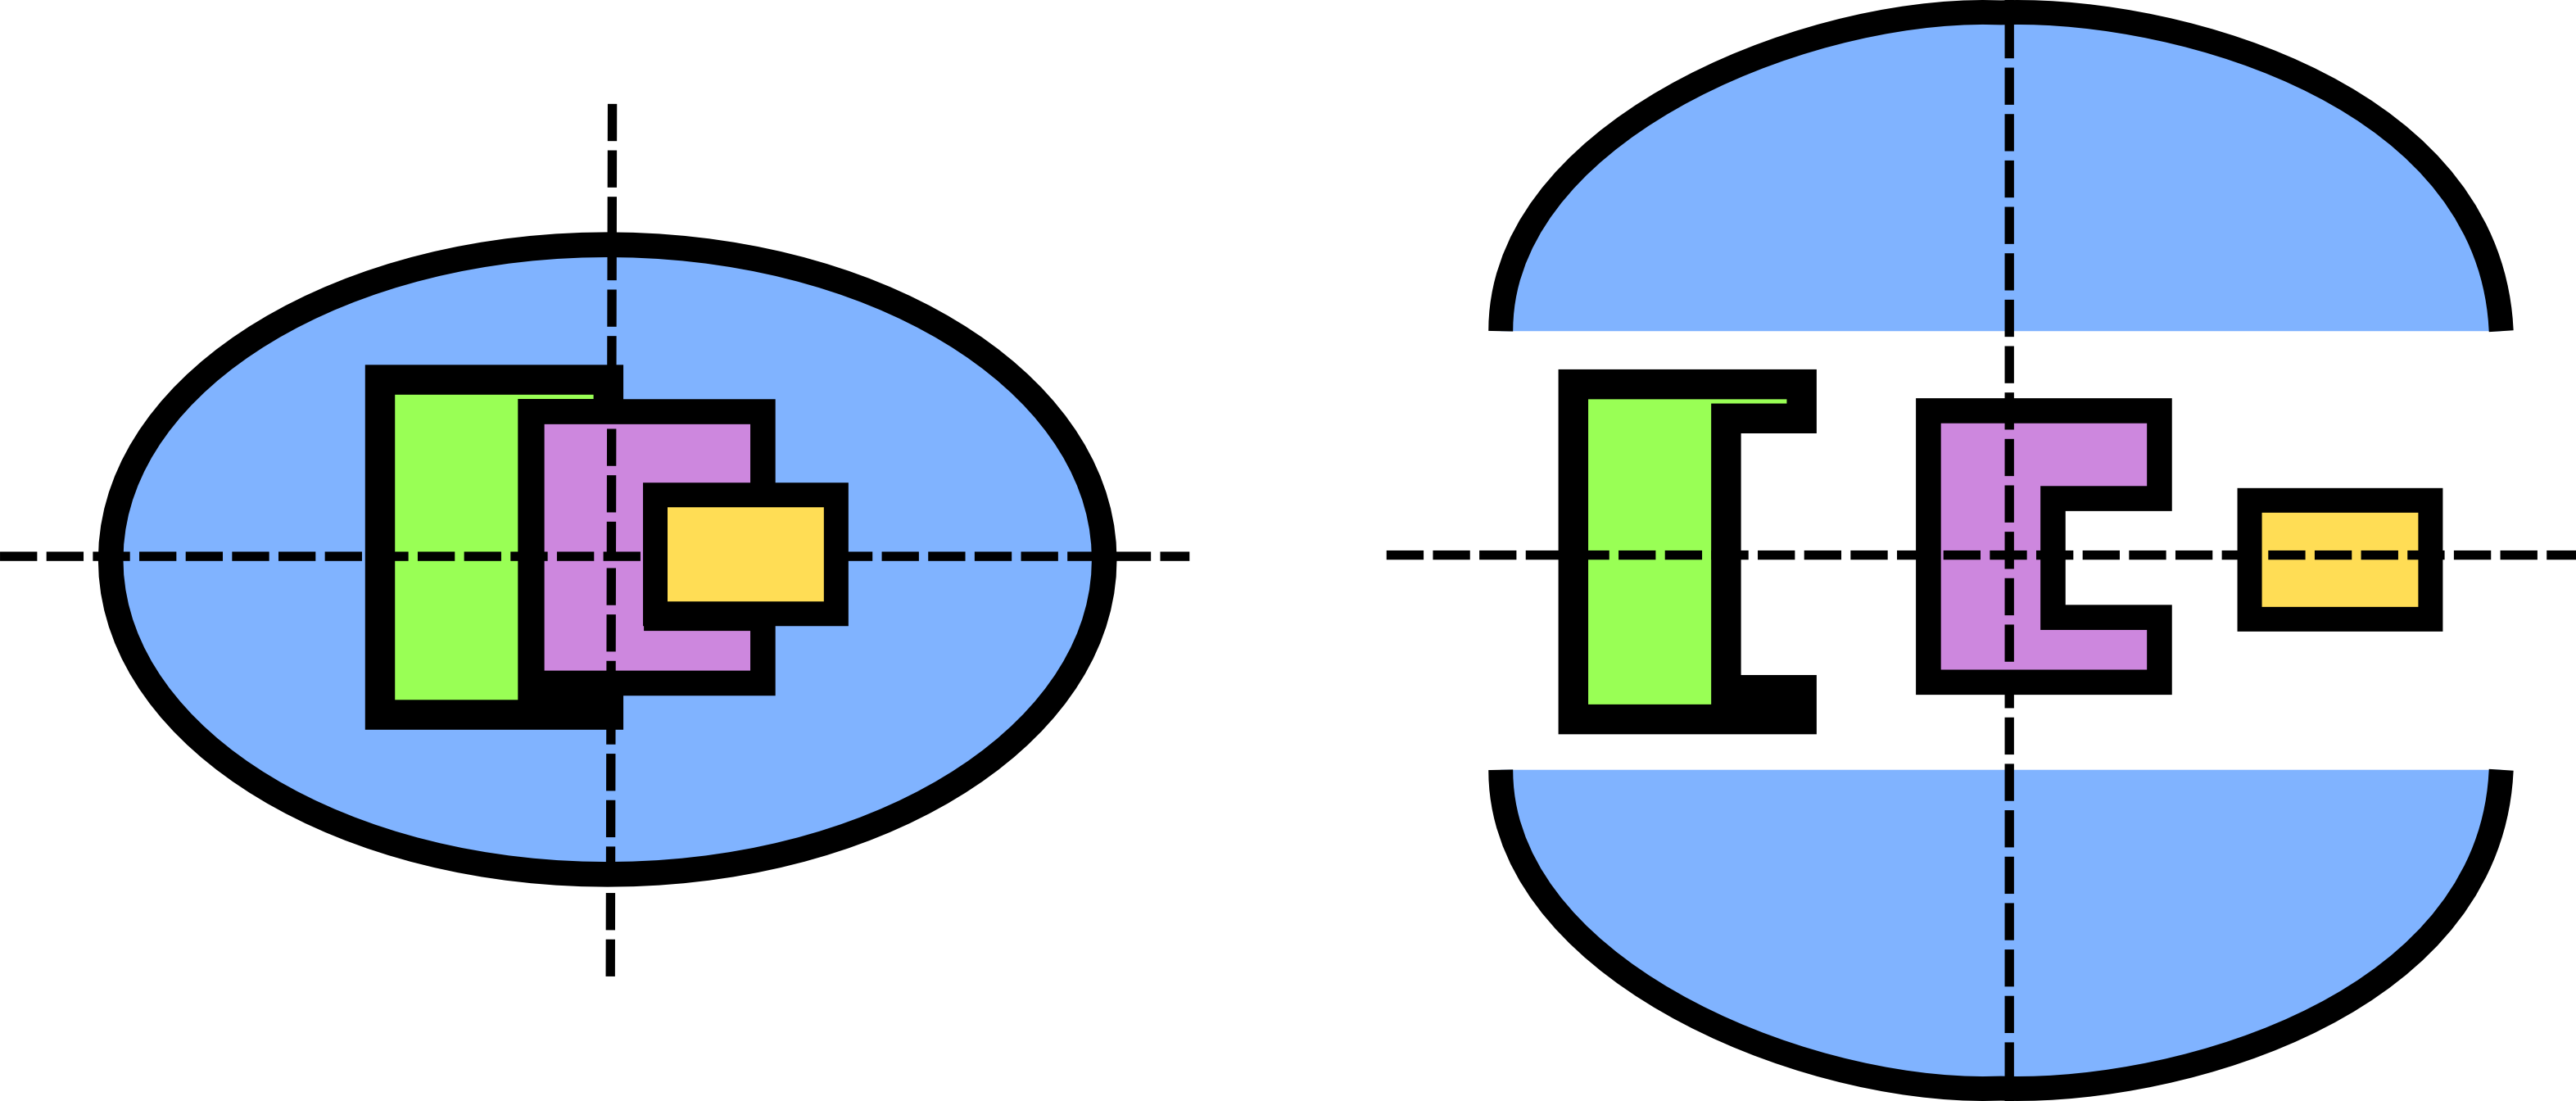
\includegraphics[width=0.7\textwidth]{chapters/figures/axes}
	\caption{The interior parts of an object are exploded in a different direction than their container}
	\label{fig:axes}
\end{figure}
In some cases, especially in the case technical visualizations e.g. assembly instructions or visual descriptions of machines the parts would block each other if they are not disassembled in the correct order and direction. A solution for this is an explosion graph representation of the Object\cite{proc:Li:2008:AGI}: Each node of this directional acyclic graph has edges pointing to parts blocking it from exploding (see \ref{fig:hierarchy}). It is generated by an algorithm, that, starting with all parts in the active set, would recursively check for unblocked parts,remove them from the active set and draw an edge from the unblocked part to any active part that would touch it.\\
To further expand the possibilities, several parts can be grouped into sub-assemblies that are then part of a hierarchical explosion graph. that has explosion graphs as nodes.\\
\begin{figure}[tb]
	\centering
	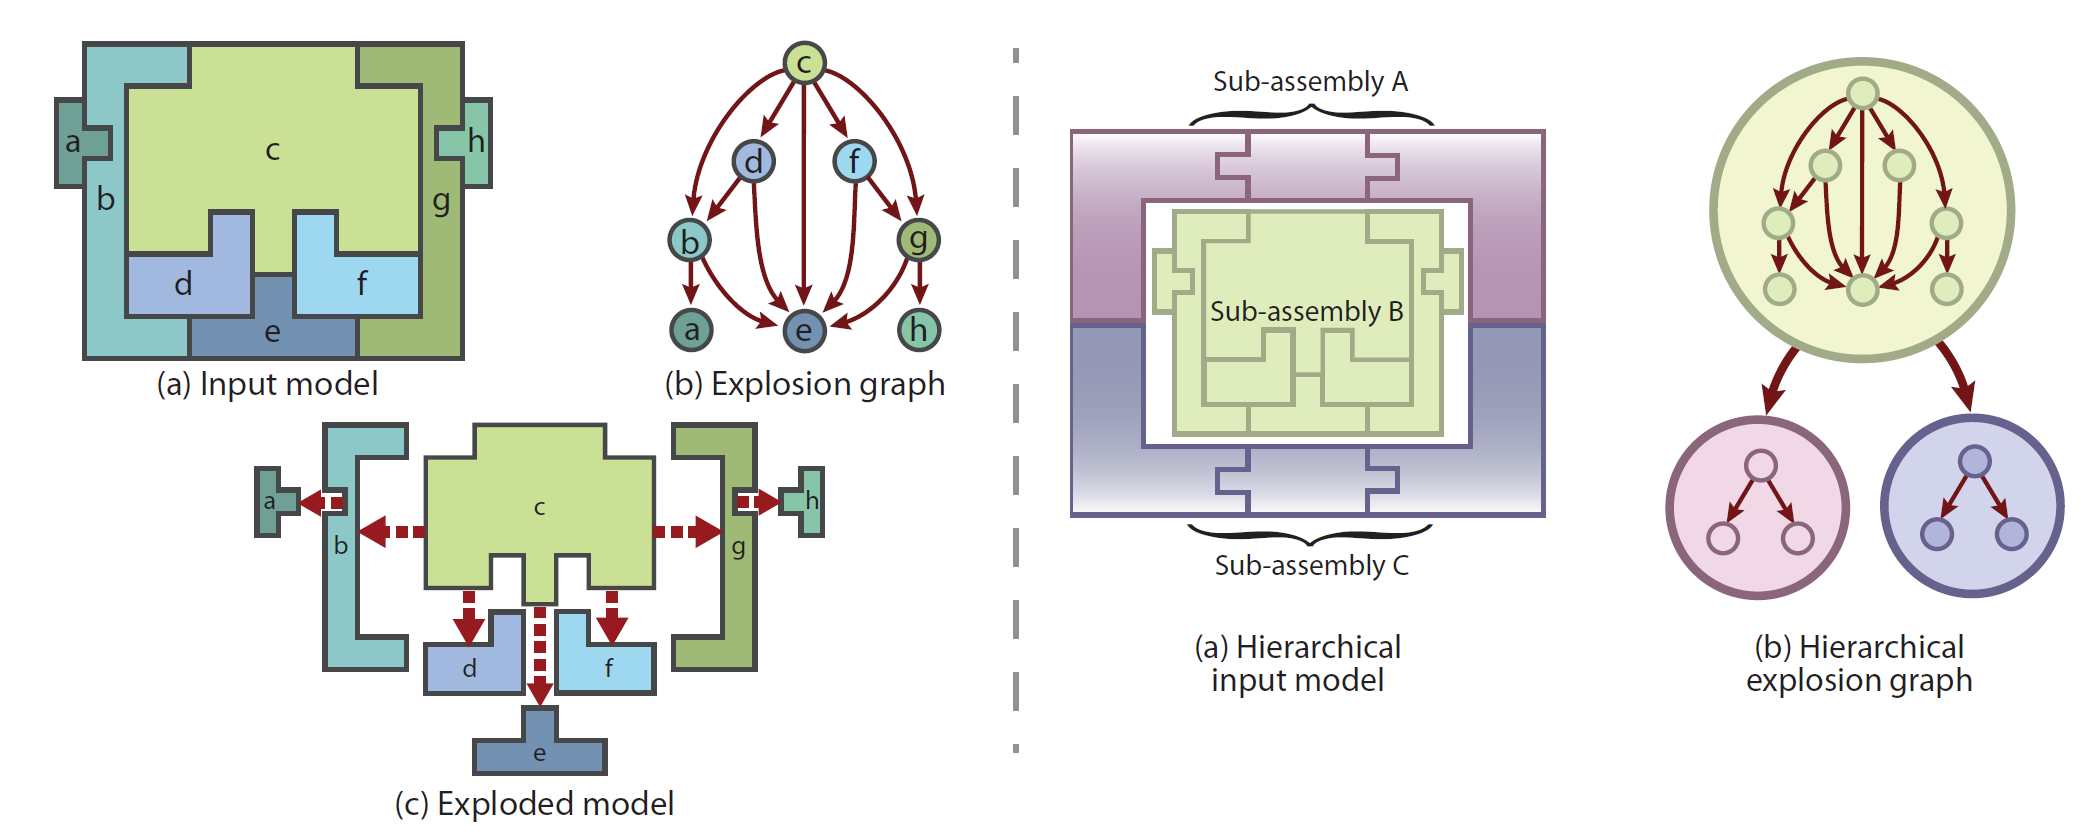
\includegraphics[width=0.7\textwidth]{chapters/figures/hierarchy}
	\caption{Explosion graph and hierarchical explosion graph\cite{proc:Li:2008:AGI}}
	\label{fig:hierarchy}
\end{figure}
If one now wanted to see a certain part of the object of interest in an exploded view, all of the parts that its edges in the explosion graph point to would have to be exploded first. If it were also part of a sub-assembly, all sub-assemblies that would have edges pointing from the part's subassembly would need to be exploded before that.
\subsection{Visibility}
Another challenge is the decision how far to displace the objects. Ideally each part should be fully visible but if there are many objects to be exploded or system the displacement direction is similar to the viewing direction, the size of the graph would grow to be enormous therefore resulting in loss of detail and expressiveness of the visualization. That may make it necessary to have some overlap as a trade-off to retain the compactness of the visualization.\\
\begin{figure}[tb]
	\centering
	\includegraphics[width=0.9\textwidth]{chapters/figures/perspective}
	\caption{The closer the viewpoint comes to the displacement axis, the larger has to be the offset to reveal the whole object of interest}
	\label{fig:perspective}
\end{figure}
With a freely rotatable and movable viewpoint the user can avoid visual clutter or lack of compactness (depending on how the system behaves) by choosing a viewpoint that provides as little clutter as possible,which narrows down the possibilities of expressive viewpoints to a minimum.\\
A solution for this would be to use a view dependent force-based displacement behavior as suggested by Bruckner and Gr\"oller\cite{proc:bruckner-2006-EVV}: Each exploding part is being displaced by a sum of multiple forces:
\begin{itemize}
\item \textbf{Explosion force} This force is pushing the part away from its original location, its magnitude is indirectly proportional to $e^{||r||}$ where $r$ is the distance between the object and the explosion point
\item \textbf{Spacing force} This repulsive force that each exploded part effects on all other exploded parts prevents parts from clustering and is indirectly proportional to $r^2$ where $r$ is the distance between the two parts.
\item \textbf{Viewing force}Additionally,  a viewing force is introduced that pushes the parts away from the viewing ray, thus preventing occlusions. It is indirectly proportional to the distance $r$ between the viewing ray and the part.
\end{itemize}
\begin{figure}[tb]
	\centering
	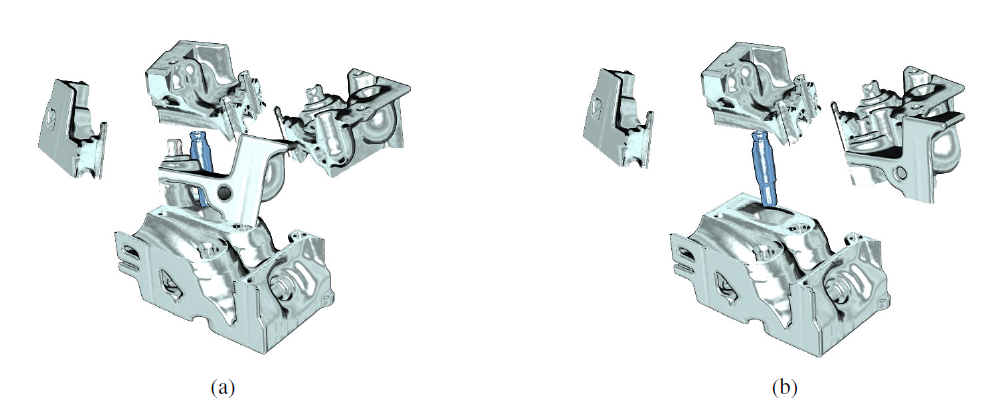
\includegraphics[width=0.7\textwidth]{chapters/figures/motor}
	\caption{(a) force-based exploded view without viewing force (interesting part is occluded) (b) with viewing force\cite{proc:bruckner-2006-EVV}}
	\label{fig:motor}
\end{figure}
This approach results in very intuitive manipulation of the graphic, making the part of the object of interest that one is looking at always visible with smooth transitions between the positions of the parts when changing viewpoints.\\
In this approach the parts don't have to explode along a predefined axis, the explosion direction can be dynamically determined by the forces, which looks impressive for anatomical data, for a technical illustration it is less desirable, for one of the key advantages of exploded views, the retention of information of a subpart's location in a system is partially lost without a clear displacement direction.\\
The solution presented in the paper is able to define axes along which to explode, this, though with similarly intuitive interaction by looking at a certain point still has the problem of little oversight when viewing from certain angles.
\subsection{Interactivity}
The biggest advantage of a computerized illustration over the classic static illustration is interactivity, most obviously the possibility to view an object from every different direction, which as described above creates its own challenges. Another aspect is the possibility for the user to choose which part of the graphic are interesting to her or him.\\
 In Li et al.'s solution\cite{proc:Li:2008:AGI} this is restricted to the predefined parts of the data sets that can be selected by clicking on them which causes the explosion to adapt, so that the selected part is fully visible. Another possibility is dragging a part along its explosion axis which causes which causes all parts on that axis to move along with it until a part that moves along a different axis is encountered. Also a 3D fish-eye viewing technique can be used that, akin to the viewing force \cite{proc:bruckner-2006-EVV} can be used to move the parts along their axes.\\
The force-based solution is -due to the use of volume data- more flexible in the definition of parts that can be exploded: the data can be freely partitioned in cuboid subspaces that can be linked by hinges or to an axis, that can be exploded by the forces three above, each of which can be varied between a 0 and a maximum value along  with the degree of explosion\\
\section{Analysis}
Since my task required creating exploded views for objects defined by triangle meshes, my approach would be rather like Li et al.'s solution, to use the groups of the mesh as the different parts of the objects which from which an object of interest would be chosen by clicking on it.\\ 
This object of interest would stay at its place in the object, while the rest of the object would be split along a cutting plane and then moved in a smooth animation to a point that would leave the object of interest fully revealed. This object would move along the axis defined by the user in a speed that is determined by how much of the Object is visible - the more the object is occluded, the faster the occluding parts move. This non-linear acceleration drew its inspiration from the before mentioned force-based approach to displacing the elements of the object, though my goal was to fully reveal the centered object, which though it normally works, is not guaranteed.\\
The biggest problem to tackle was now how to handle viewing directions that cause the graphic to grow up to -in th worst case- infinity.\\
Neither the prospect of visual clutter, indeterminate explosion directions nor the idea of a graphic that would grow infinitely when viewed from the wrong angle proved satisfactory, especially from a usability standpoint: Though the system allows for a freely movable viewpoint, most perspectives just deliver unsatisfactory or even useless results.\\
Since a maximum threshold for the explosion along an axis was inevitable, my intention was to keep it low enough to retain a satisfactory level of compactness I chose ghosting as a technique to still convey information about the object of interest to the user when it was occluded by another part of the object.
\subsection{Ghosting}
As the exploded view, ghosting is a smart visibility technique to illustrate the normally occluded inner workings of a complex object. In this case smart visibility is defined like this.
\begin{quote}Smart Visibility considers more than just light propagation. For example also the relevance of the individual objects is taken into account. An important object might shine through an otherwise occluding object closer to the viewer. \cite{Viola-05-Smart}\end{quote}
The advantages of this technique are that the in contrast to the exploded view, objects visualized with ghosting do not take up more space than the objects themselves. Additionally, the inner parts of an object are shown at their actual position inside the object, thus being able to show the composition of an object accurately than an Exploded view might be able to do.\\
On the other Hand, ghosted views are usually more cluttered because of this, which can lead to loss of detail and insight. Also they tend to look confusing in case two objects are in between the viewer and the object of interest. To avoid these problems and achieve good results the following rules should be considered:\cite{Viola-05-Smart}
\begin{itemize}
\item faces of transparent objects never shine through
\item objects occluded by two transparent objects do not shine through
\item transparency falls-off close to the edges of transparent objects
\end{itemize}


